\newpage
\chapter{Sensitivity Analysis} \label{ch:sensitivity}



\begin{figure}[H]
\begin{subfigure}[t]{0.33\textwidth}
    \centering
    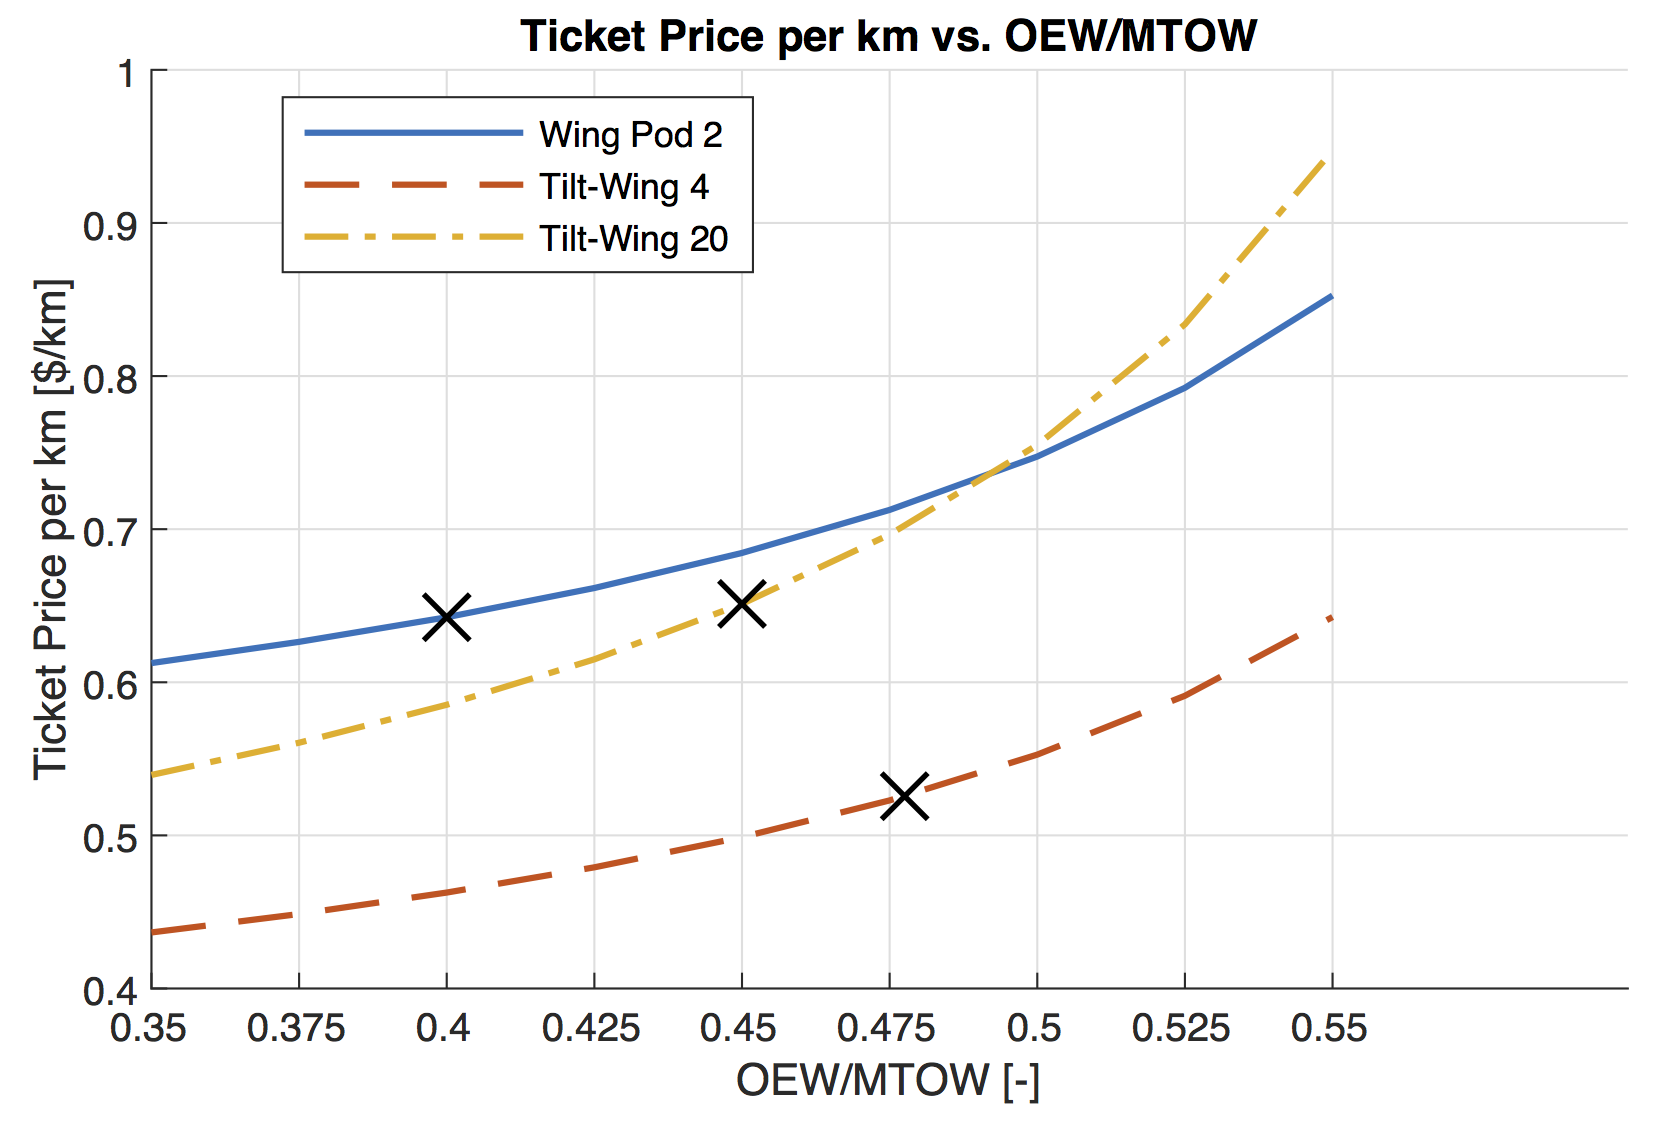
\includegraphics[width=\textwidth]{Figures/OEWMTOW_TPrice_perkmNOPAD.png}
    \captionsetup{width=.8\linewidth}
    \caption{OEW/MTOW}
    \label{fig:sens1}
\end{subfigure}
\begin{subfigure}[t]{0.33\textwidth}
    \centering
    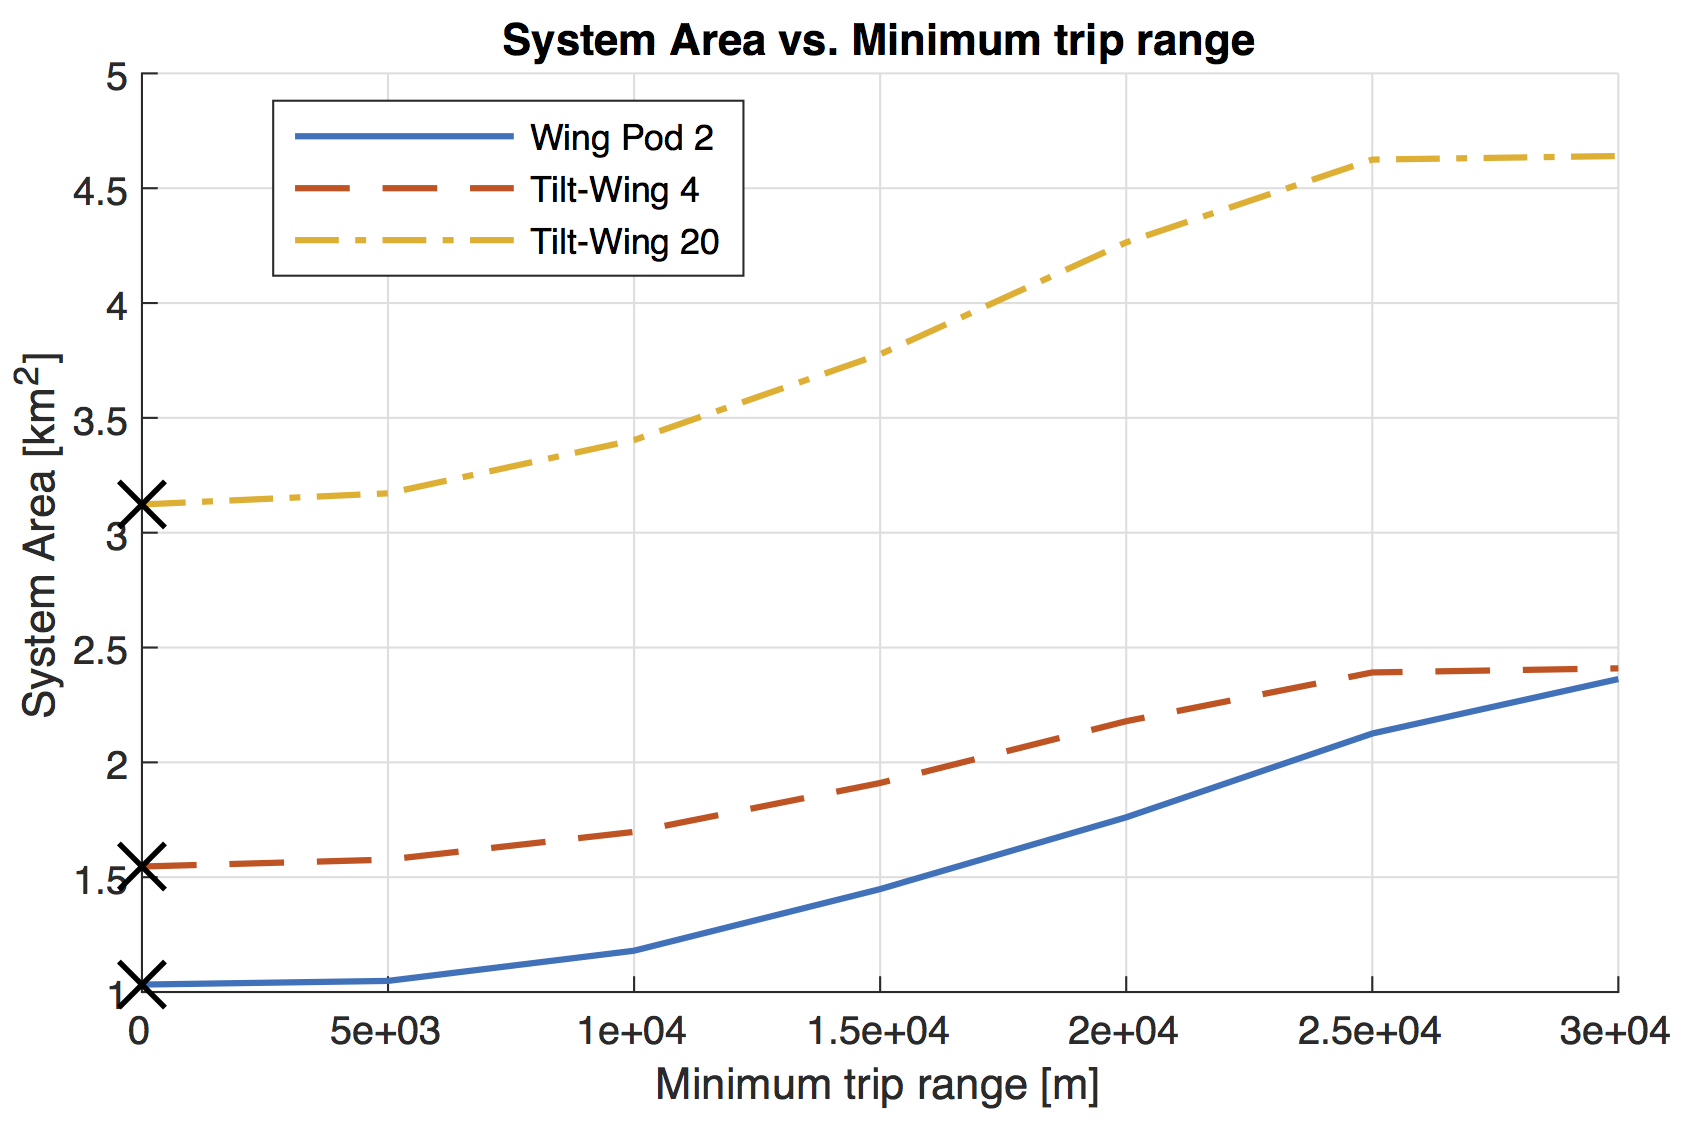
\includegraphics[width=\textwidth]{Figures/report_sys_area.png}
    \captionsetup{width=.8\linewidth}
    \caption{}
    \label{fig:sens2}
\end{subfigure}
\begin{subfigure}[t]{0.33\textwidth}
    \centering
    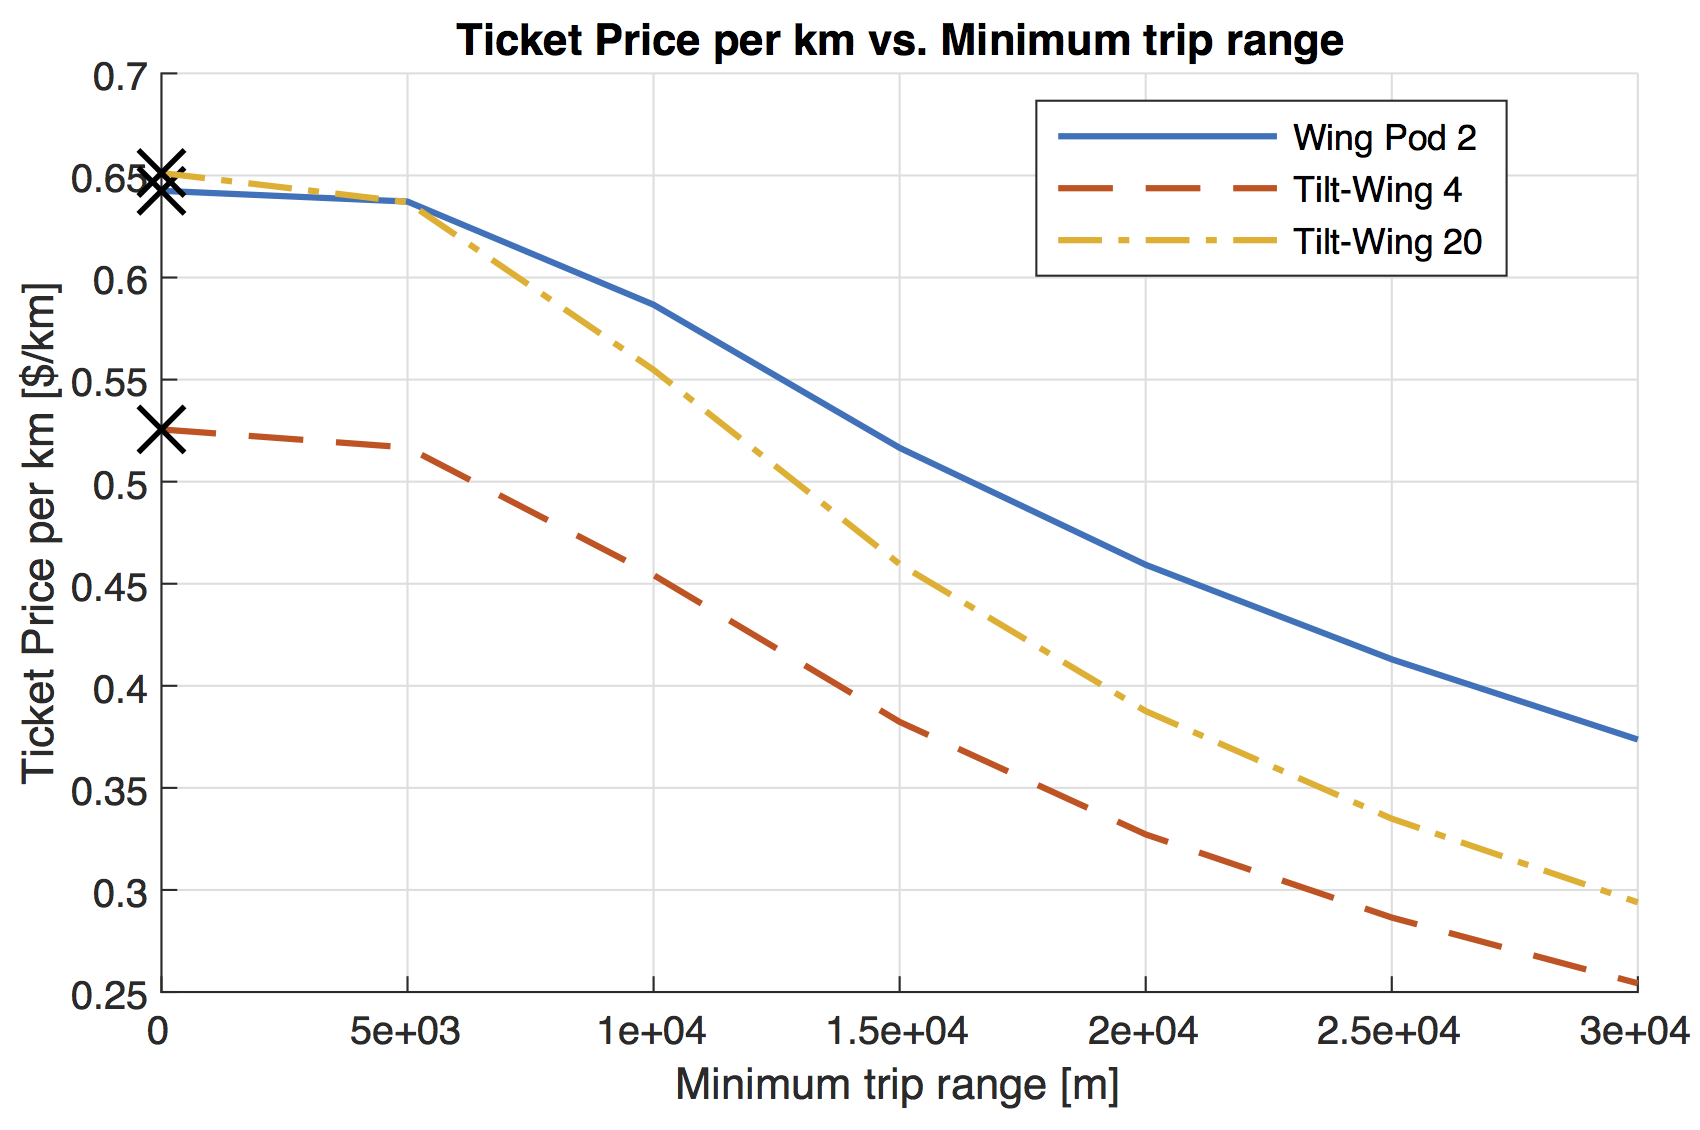
\includegraphics[width=\textwidth]{Figures/minRange_TPrice_perkmNOPAD.png}
    \captionsetup{width=.8\linewidth}
    \caption{}
    \label{fig:sens3}
\end{subfigure}
\label{fig:sens123}
\end{figure}


\begin{figure}[H]
\begin{subfigure}[t]{0.33\textwidth}
    \centering
    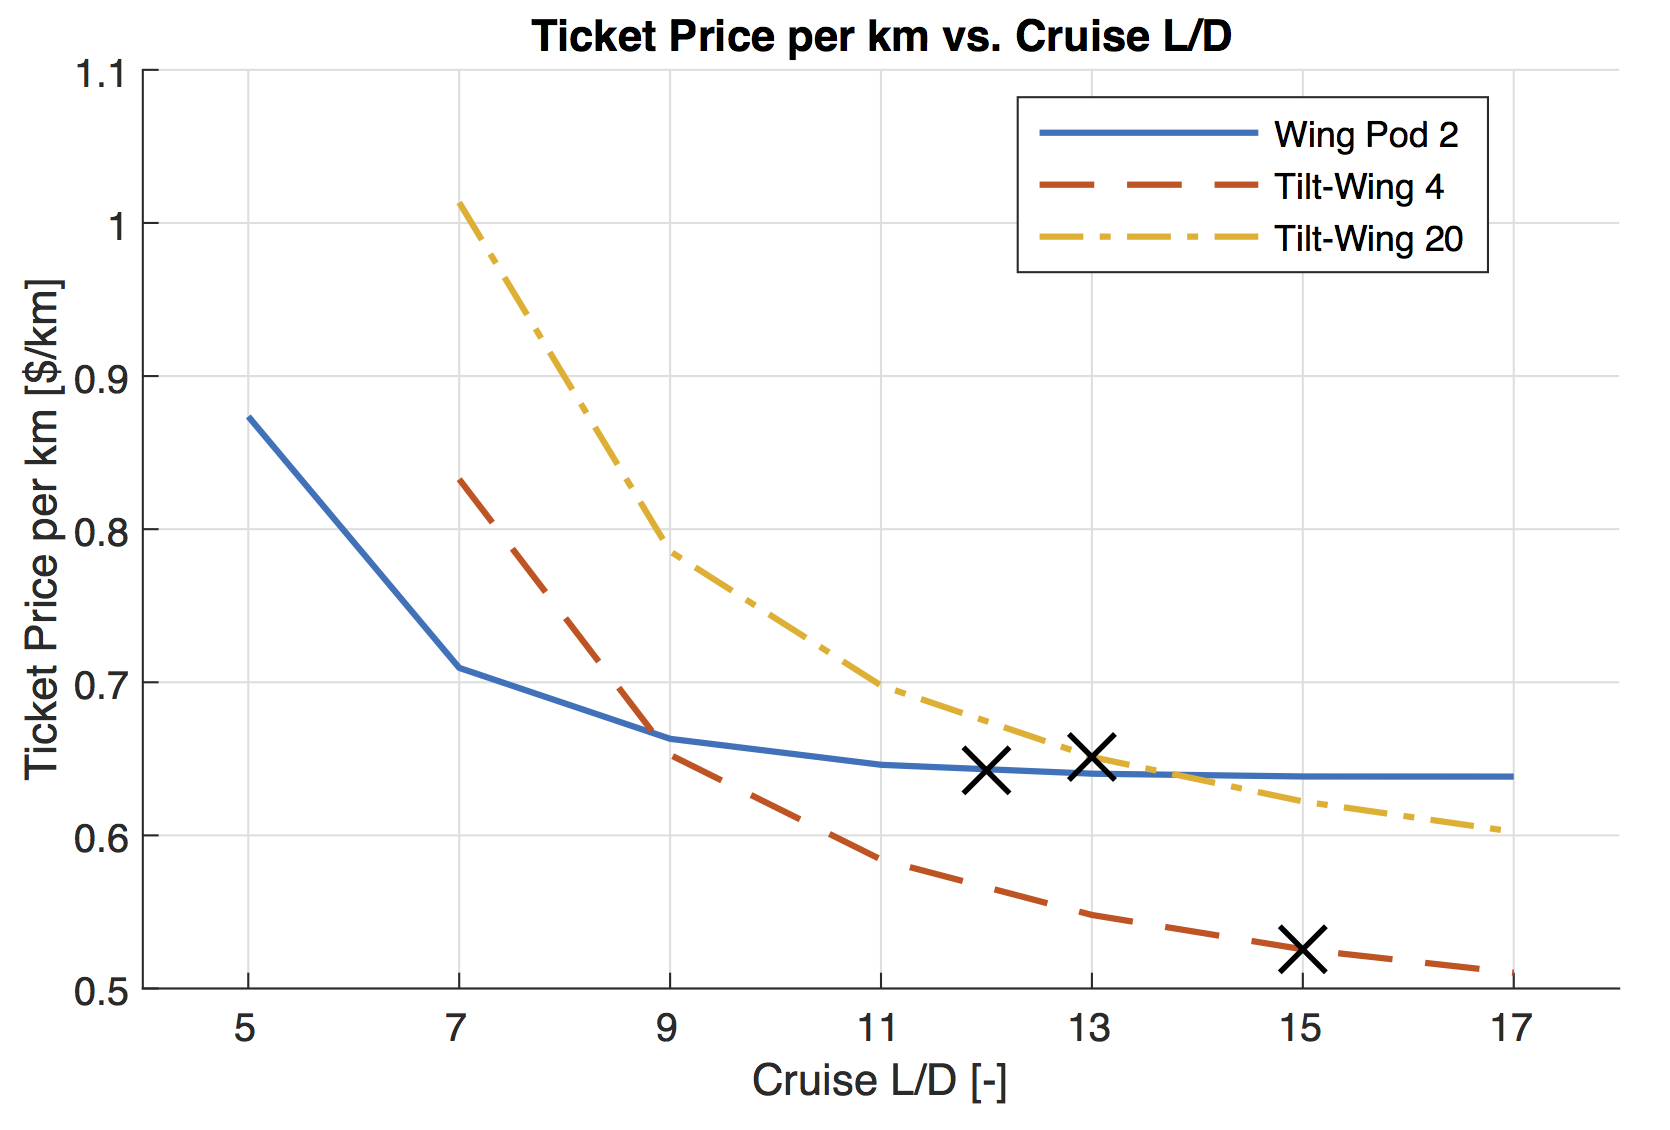
\includegraphics[width=\textwidth]{Figures/LoD_TPrice_perkmNOPAD.png}
    \captionsetup{width=.8\linewidth}
    \caption{OEW/MTOW}
    \label{fig:sens4}
\end{subfigure}
\begin{subfigure}[t]{0.33\textwidth}
    \centering
    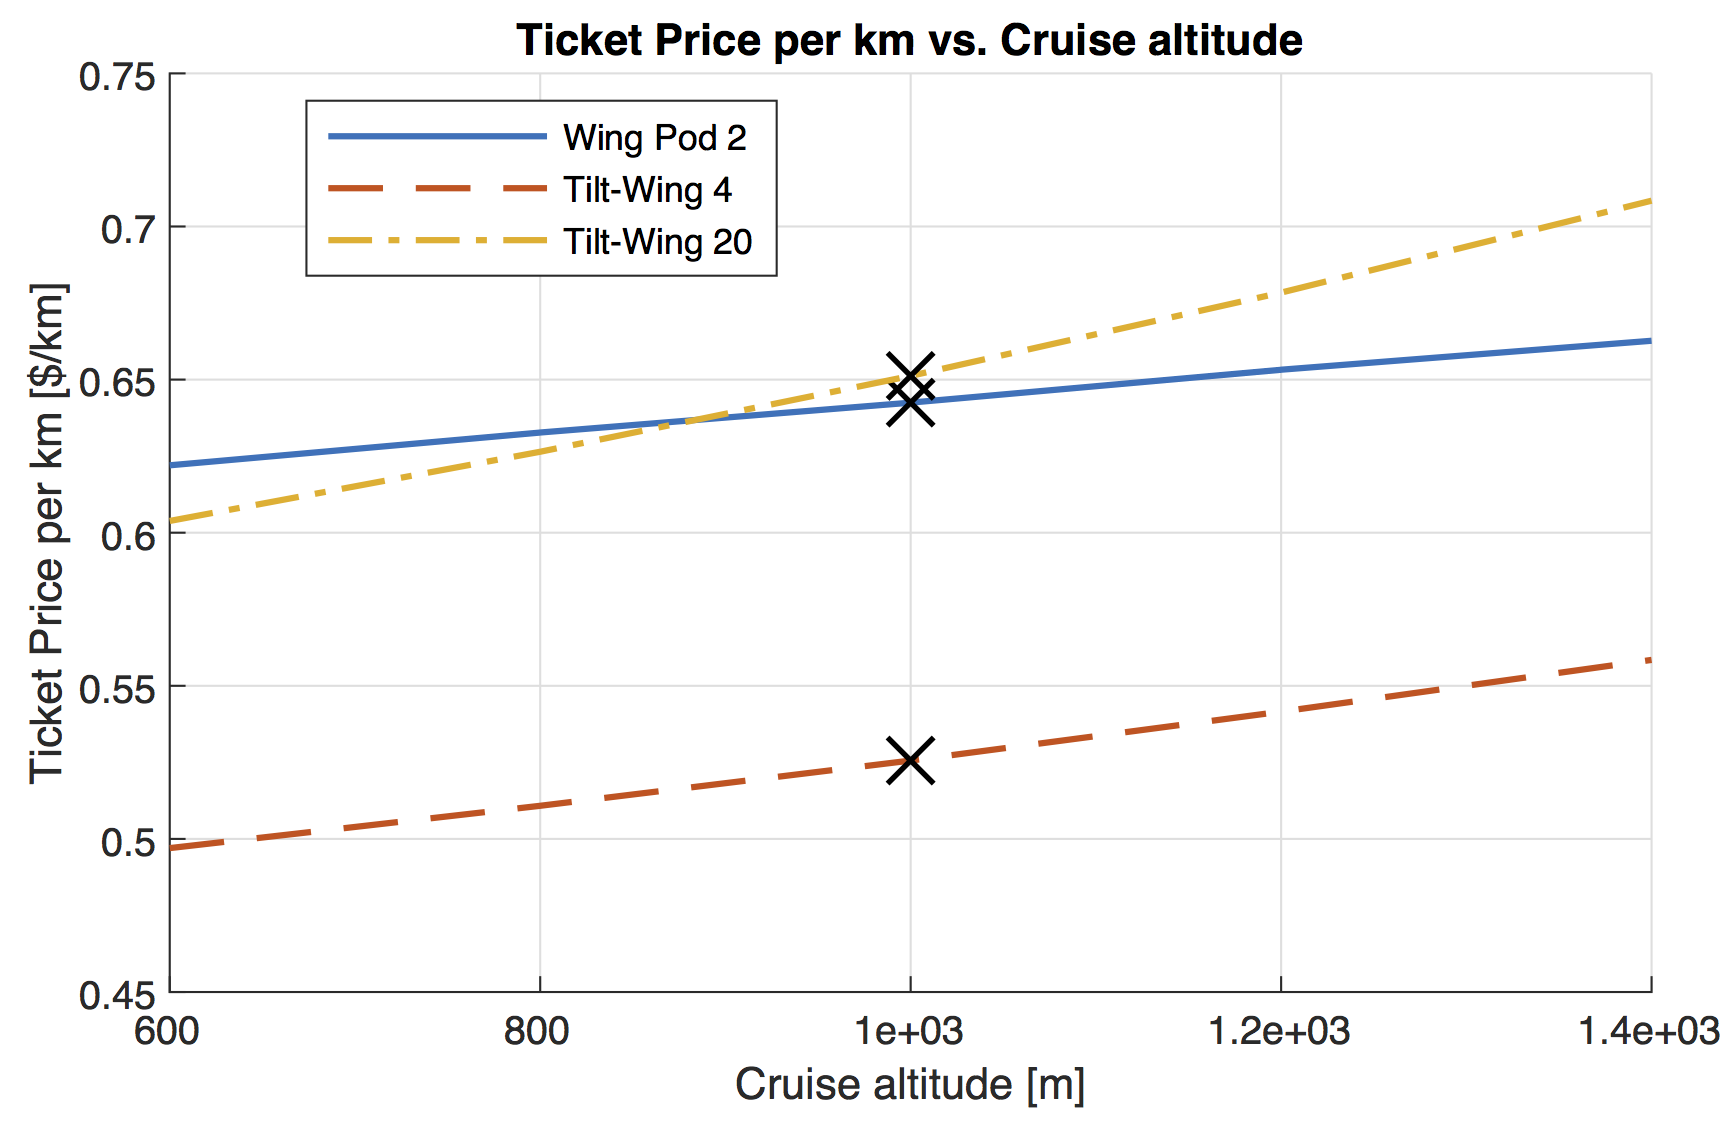
\includegraphics[width=\textwidth]{Figures/Alt_TPrice_perkmNOPAD.png}
    \captionsetup{width=.8\linewidth}
    \caption{}
    \label{fig:sens5}
\end{subfigure}
\begin{subfigure}[t]{0.33\textwidth}
    \centering
    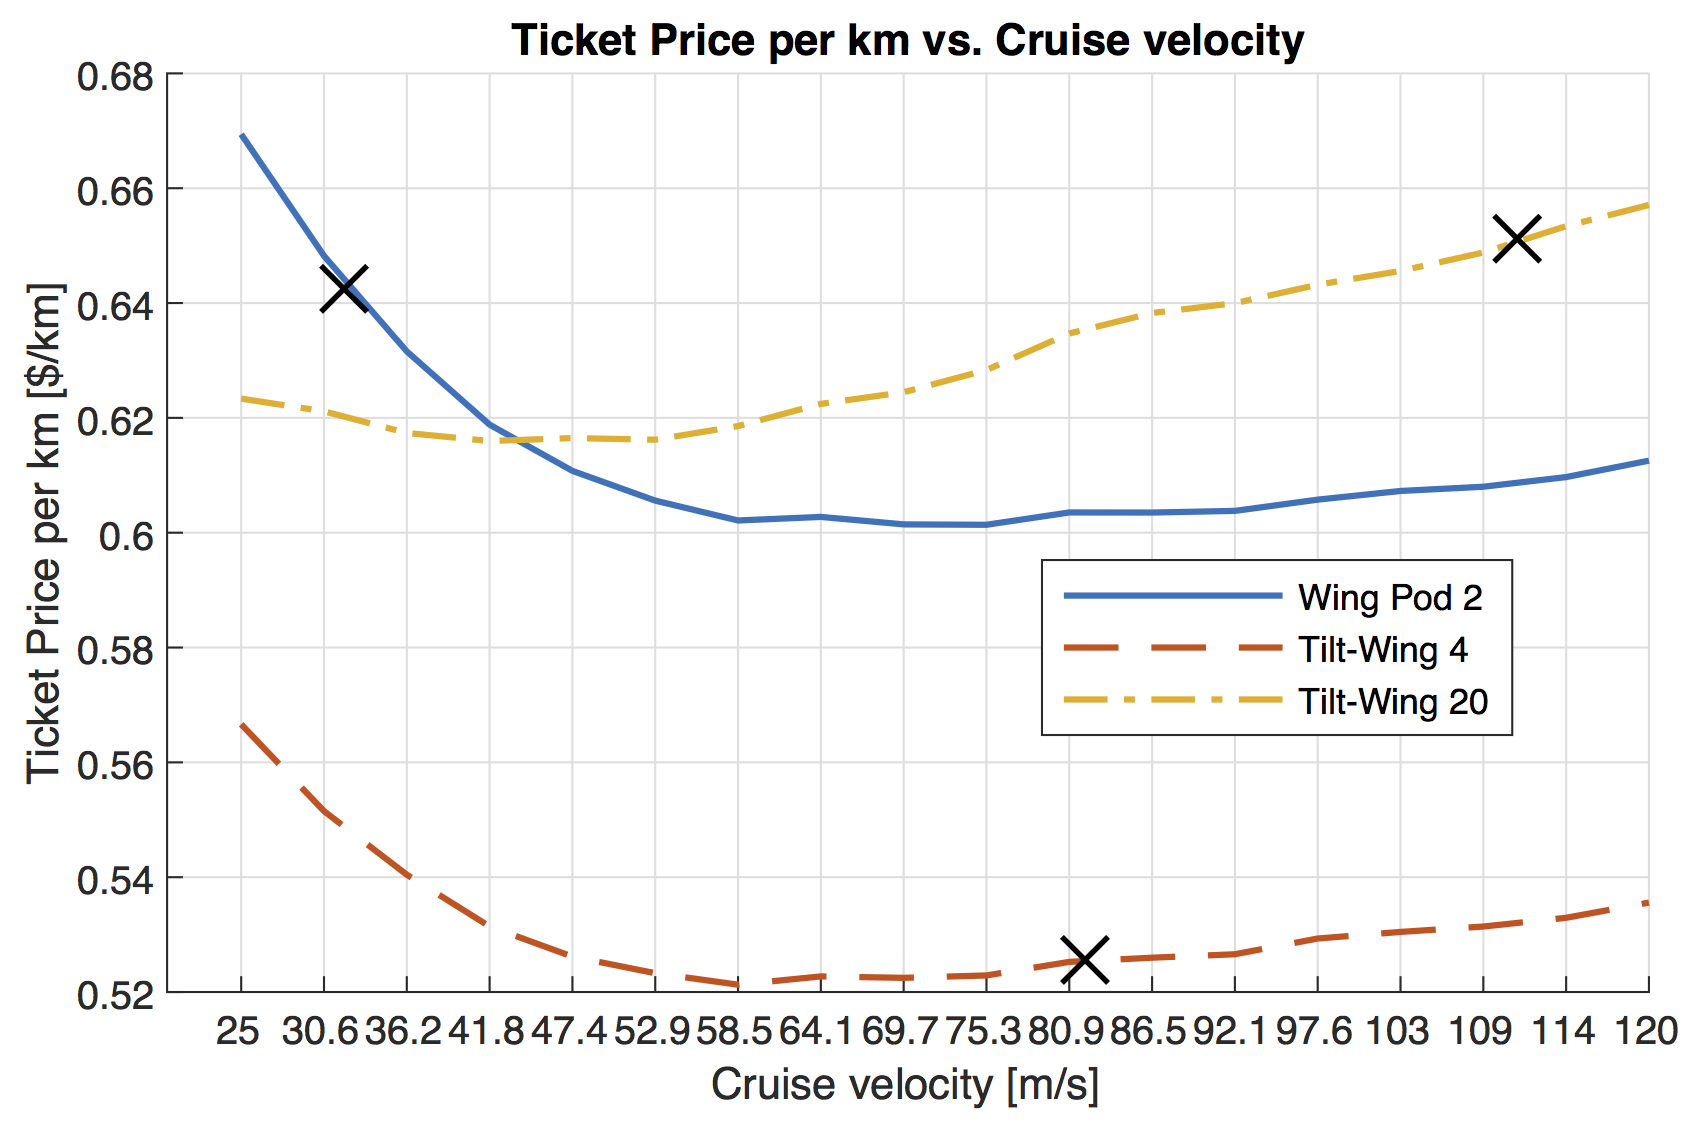
\includegraphics[width=\textwidth]{Figures/Cruise_TPrice_perkmNOPAD.png}
    \captionsetup{width=.8\linewidth}
    \caption{}
    \label{fig:sens6}
\end{subfigure}
\label{fig:sens456}
\end{figure}

\begin{figure}[H]
\begin{subfigure}[t]{0.33\textwidth}
    \centering
    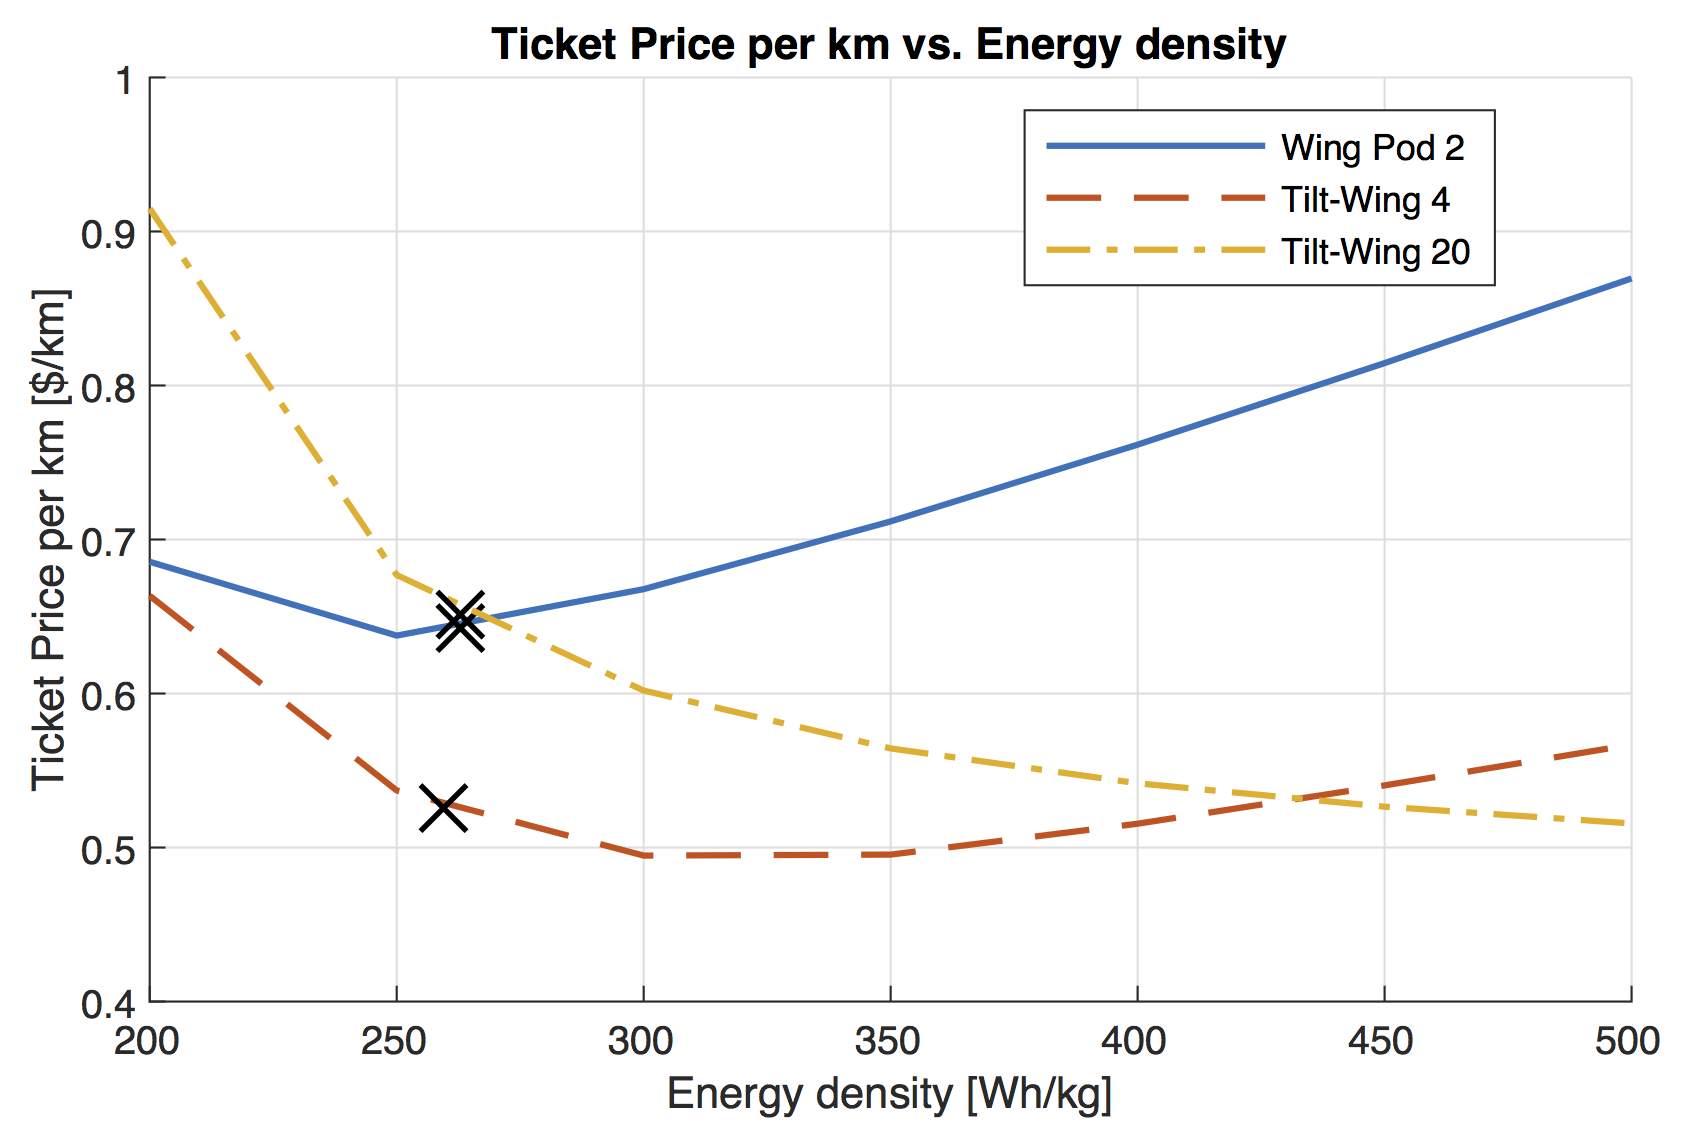
\includegraphics[width=\textwidth]{Figures/Edens_TPrice_perkmNOPAD.png}
    \captionsetup{width=.8\linewidth}
    \caption{OEW/MTOW}
    \label{fig:sens7}
\end{subfigure}
\begin{subfigure}[t]{0.33\textwidth}
    \centering
    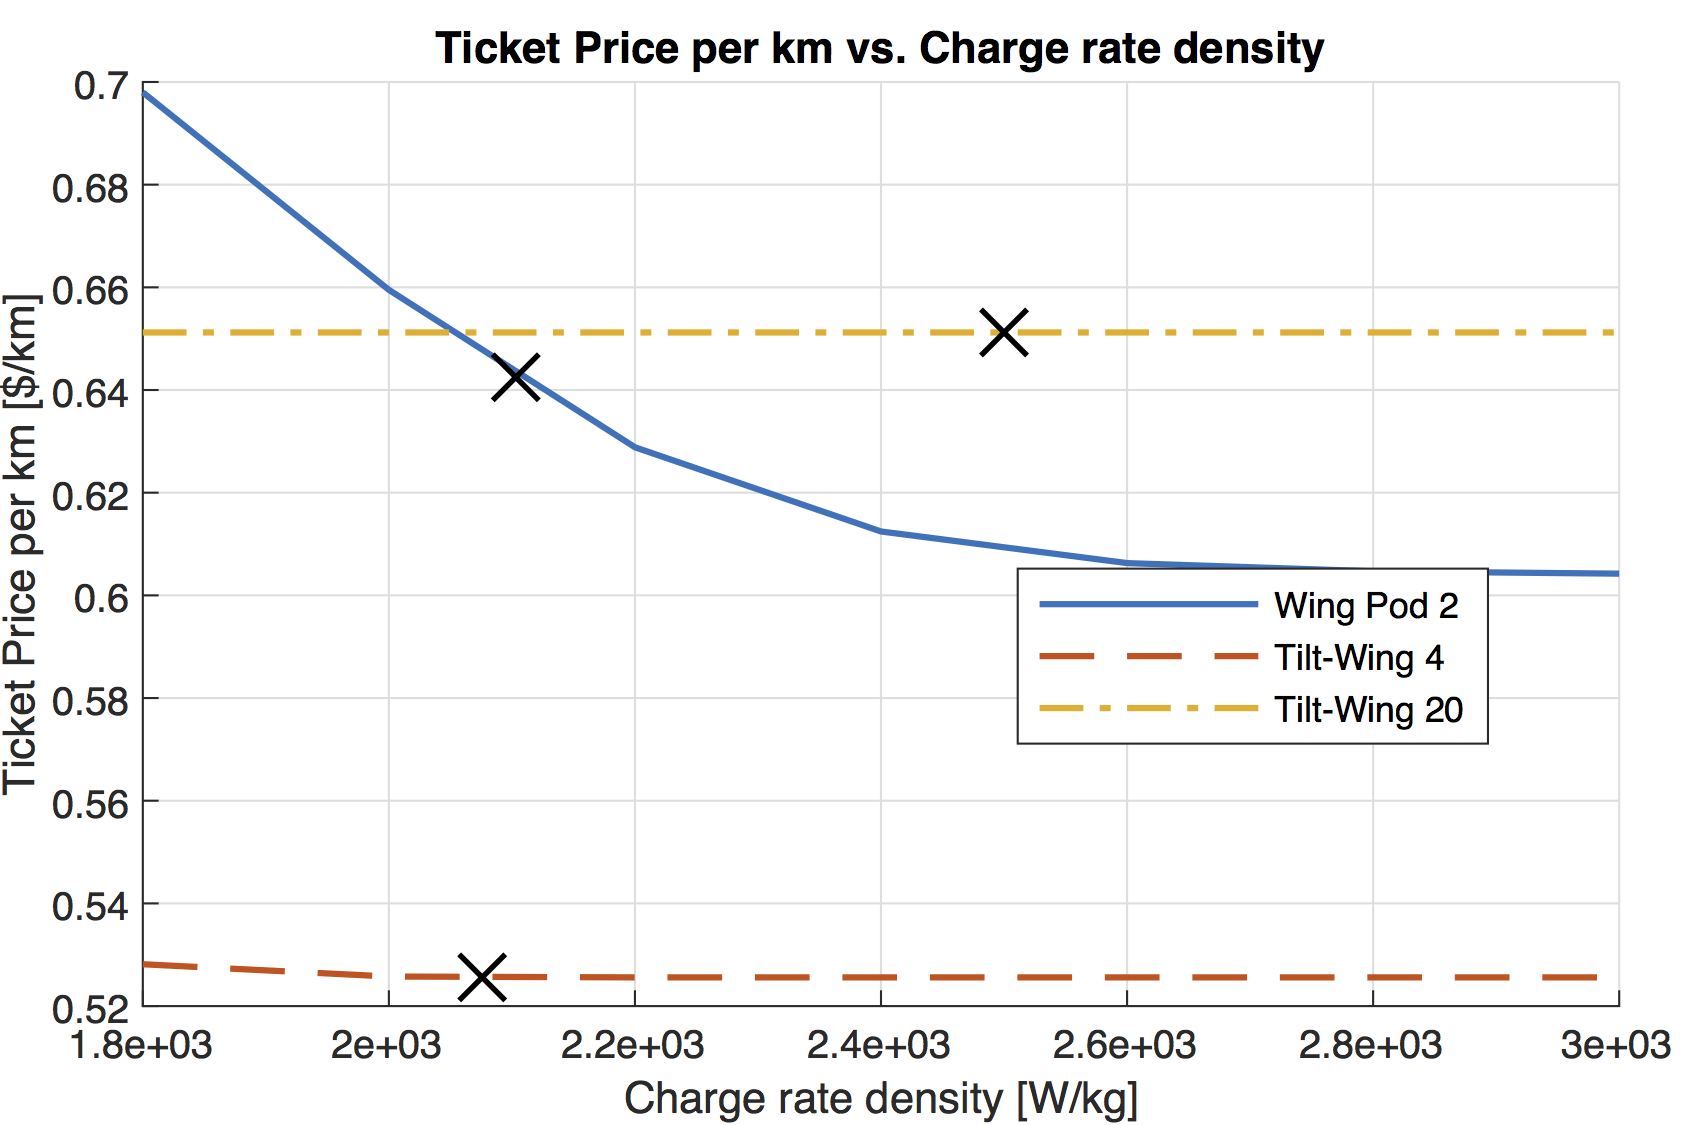
\includegraphics[width=\textwidth]{Figures/CRate_TPrice_perkmNOPAD.png}
    \captionsetup{width=.8\linewidth}
    \caption{}
    \label{fig:sens8}
\end{subfigure}
\begin{subfigure}[t]{0.33\textwidth}
    \centering
    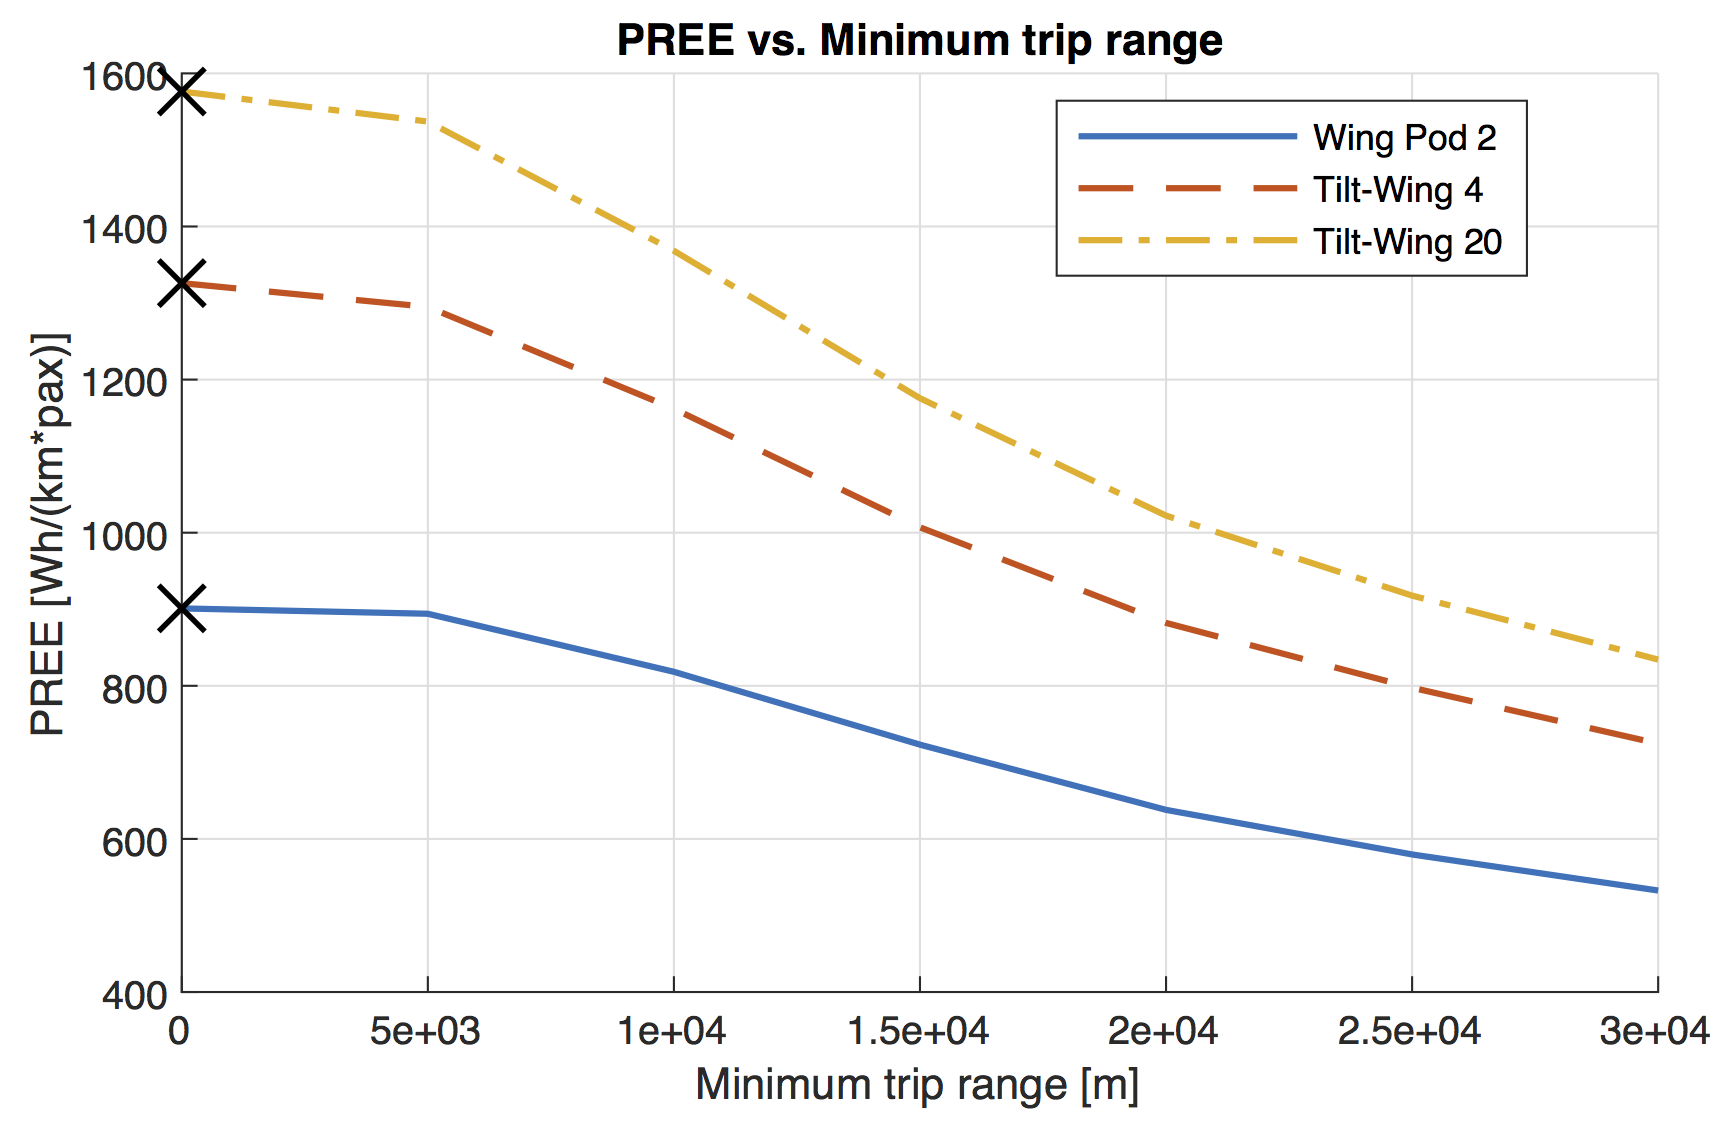
\includegraphics[width=\textwidth]{Figures/report_PREE.png}
    \captionsetup{width=.8\linewidth}
    \caption{}
    \label{fig:sens9}
\end{subfigure}
\label{fig:sens789}
\end{figure}

\subsection{Autonomous and Remotely Assisted Piloting}

\begin{wrapfigure}[18]{r}{0.35\textwidth}
    \centering
    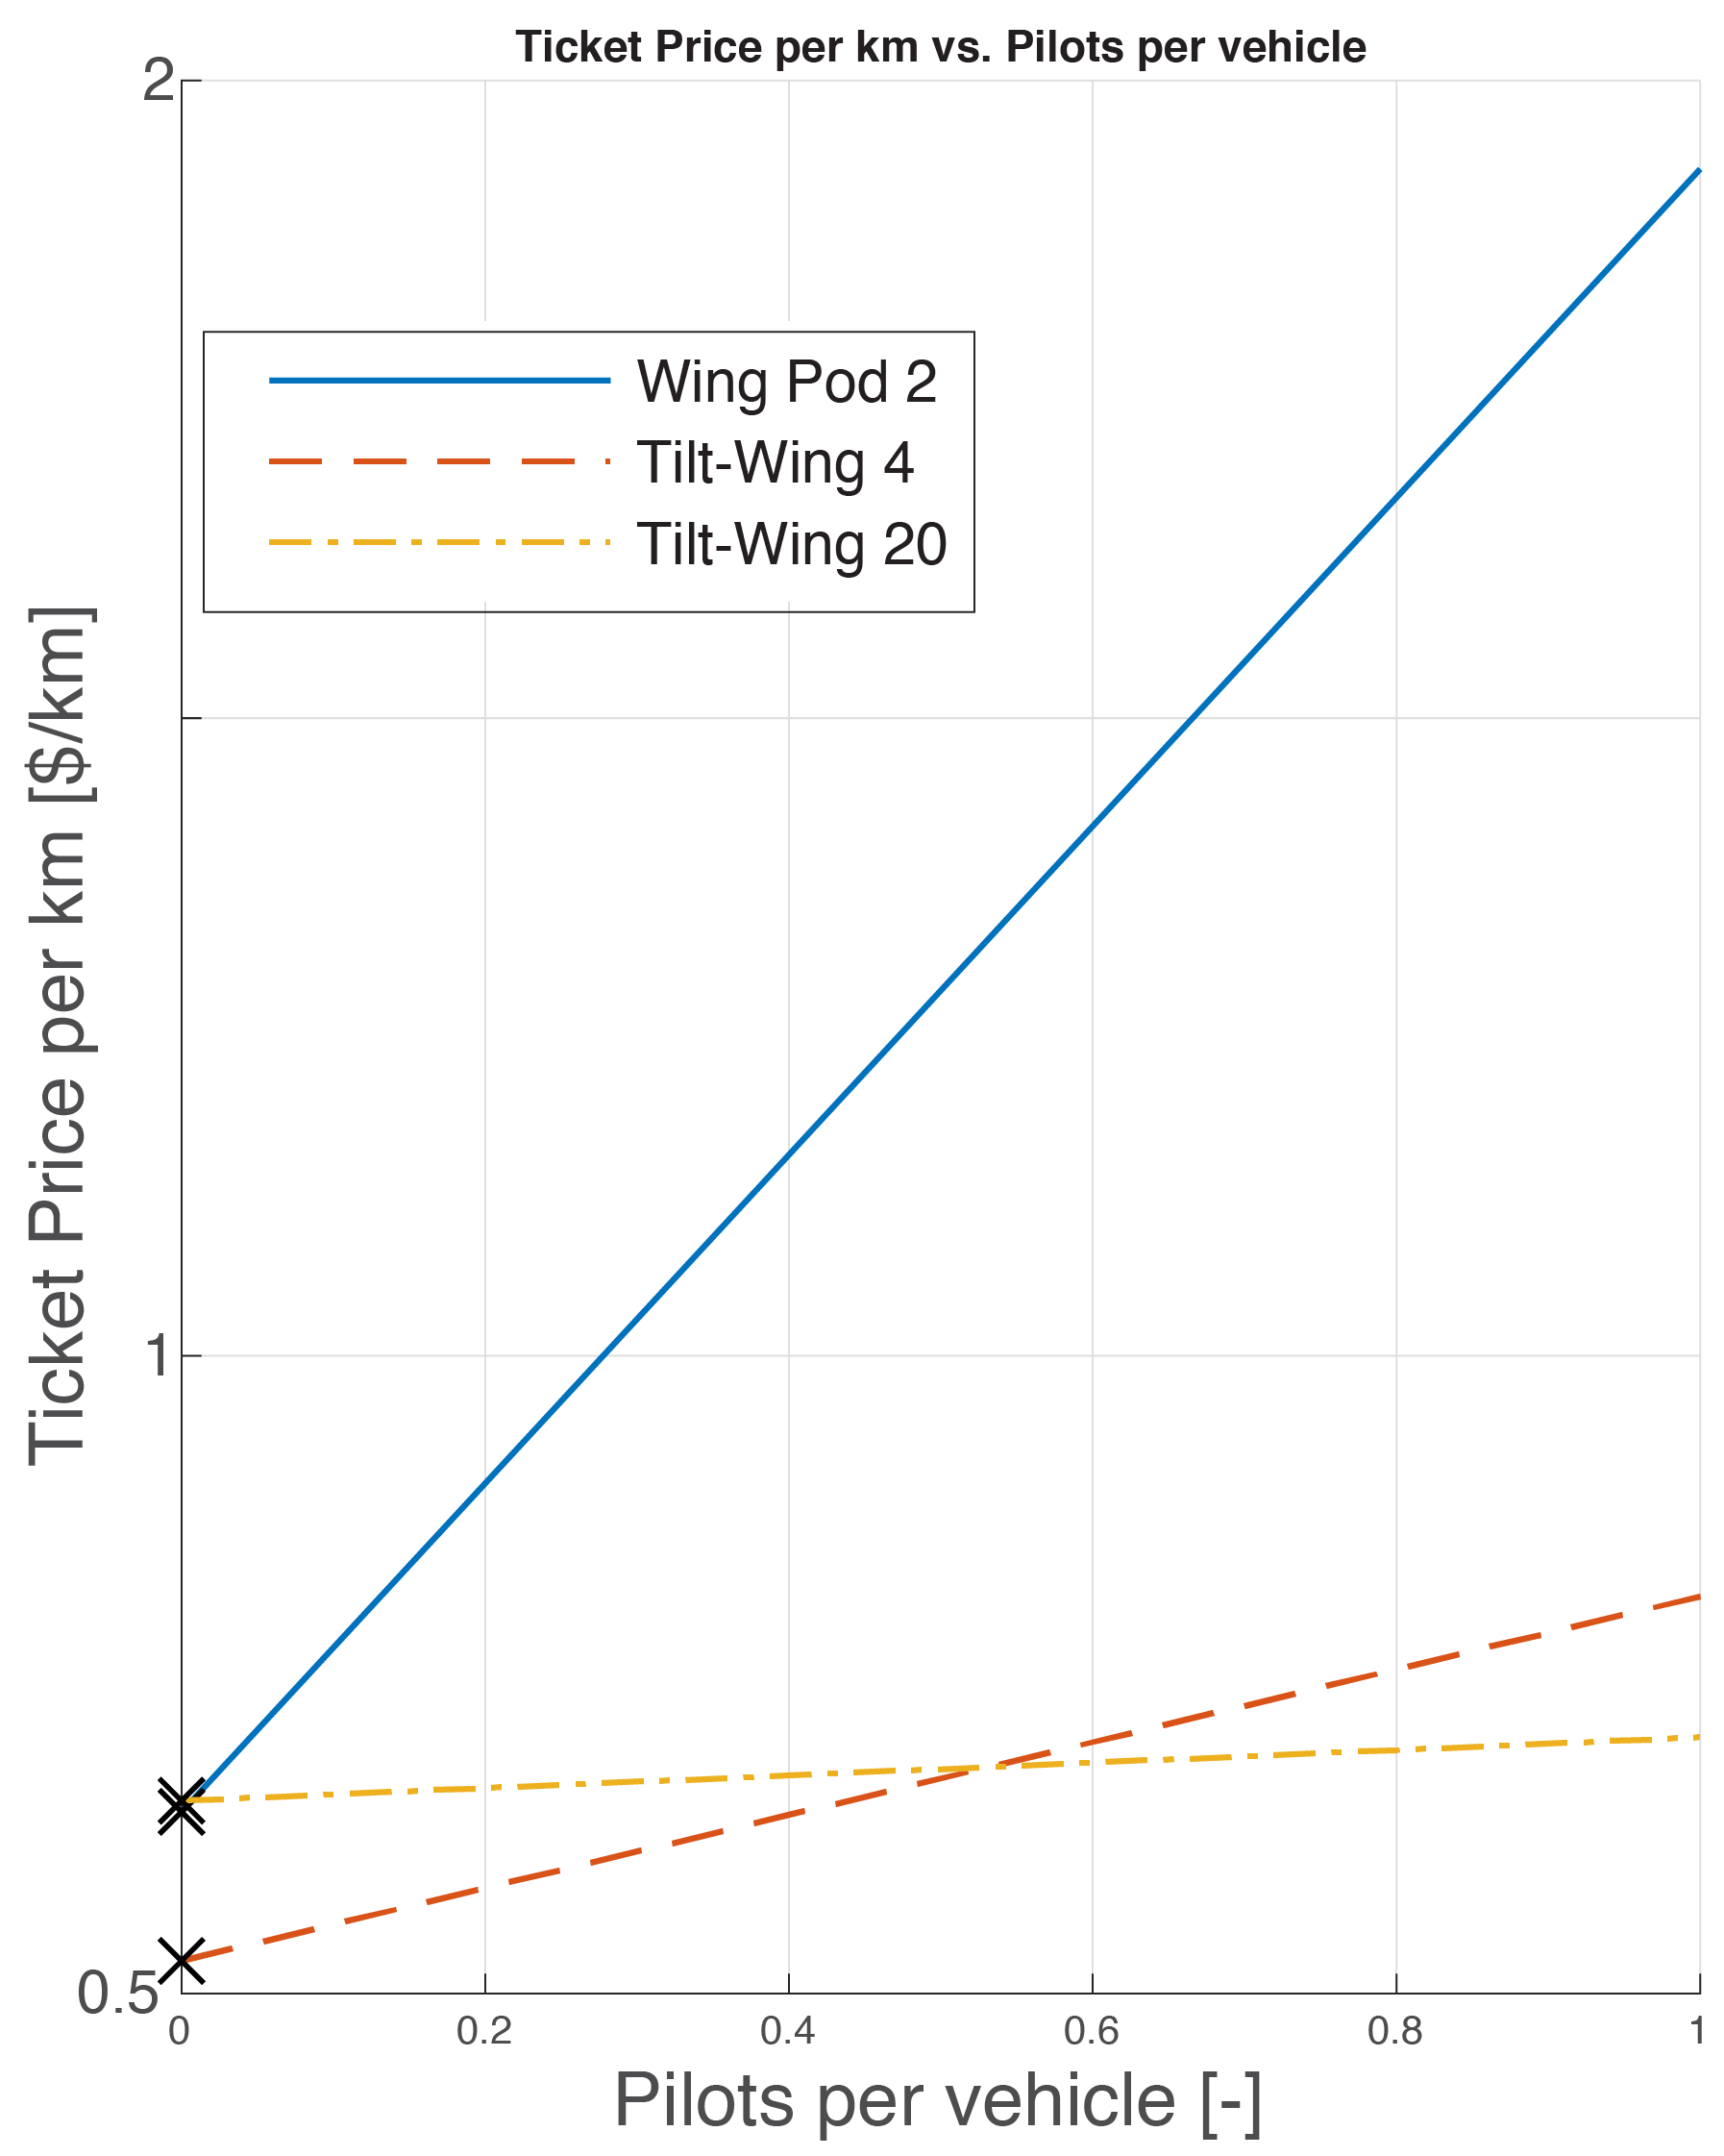
\includegraphics[width=0.35\textwidth]{Figures/autonomous_TPrice_perkm.png}
    \caption{Ticket price increase due to including remote pilots, to assist autonomous vehicles.}
    \label{fig:autocost}
\end{wrapfigure}

Much of the trade-off has been done assuming that all the vehicles are completely autonomous. It is likely that remote piloting capabilities will be necessary for safety reasons. A pilot may need to intervene in certain situations. This also helps with a feeling of comfort for passengers. By completing a sensitvity study based on the 
